%%%%%%%%%%%%%%%%%%%%%%%%%%%%%%%%%%%%%%%%%%%%%%%%%%%%%%%%%%%%%%%%%%%%%%%
% Sample template for MIT Junior Lab Student Written Summaries
% Available from http://web.mit.edu/8.13/samplepaper/sample-paper.tex
%
% Last Updated June 20, 2004
%
% Adapted from the American Physical Societies REVTeK-4 Pages
% at http://publish.aps.org
%
% ADVICE TO STUDENTS: Each time you write a paper, start with this
%    template and save under a new filename.  If convenient, don't
%    erase unneeded lines, just comment them out.  Often, they
%    will be useful containers for information.
%%%%%%%%%%%%%%%%%%%%%%%%%%%%%%%%%%%%%%%%%%%%%%%%%%%%%%%%%%%%%%%%%%%%%%%

%%%%%%%%%%%%%%%%%%%%%%%%%%%%%%%%%%%%%%%%%%%%%%%%%%%%%%%%%%%%%%%%%%%%%%%
% PREAMBLE
% The preamble of a LaTeX document is the set of commands that precede
% the \begin{document} line.  It contains a \documentclass line
% to load the REVTeK-4 macro definitions and various \usepackage
% lines to load other macro packages.
%
% ADVICE TO STUDENTS: This preamble contains a suggested set of
%     class options to generate a ``Junior Lab'' look and feel that
%     facilitate quick review and feedback from one's peers, TA's
%     and section instructors.  Don't make substantial changes without
%     first consulting your section instructor.
%%%%%%%%%%%%%%%%%%%%%%%%%%%%%%%%%%%%%%%%%%%%%%%%%%%%%%%%%%%%%%%%%%%%%%%

\documentclass[aps,twocolumn,secnumarabic,nobalancelastpage,amsmath,amssymb,
    nofootinbib]{revtex4}
    
    % nofootinbib is another document class option that allows you to put
    % footnotes on the page where they occur rather than at the end of the
    % paper.  This makes for easier reading!
    
    % secnumarabic is a particularly nice way of identifying sections by
    % number to aid electronic review and commentary.
    
    % amsmath and amssymb are necessary for the subequations environment
    % among others
    
    \usepackage{graphics}      % standard graphics specifications
    \usepackage{graphicx}      % alternative graphics specifications
    \usepackage{longtable}     % helps with long table options
    \usepackage{url}           % for on-line citations
    \usepackage{bm}            % special 'bold-math' package
    \usepackage[utf8]{inputenc} % para poder poner tildes
    \usepackage{siunitx}        % para las unidades
                                                                 
    %%%%%%%%%%%%%%%%%%%%%%%%%%%%%%%%%%%%%%%
    %                                 %%%%%
    % And now, begin the document...  %%%%%
    %                                 %%%%%
    %%%%%%%%%%%%%%%%%%%%%%%%%%%%%%%%%%%%%%%
    
    \begin{document}
    \title{Implementación de una librería para la detección y el análisis de interacciones de partículas con CMOS}
    \author         {Darío Federico Balmaceda}
    \email          {leschatten@gmail.com}
    %\homepage       {http://fisica.cab.cnea.gov.ar/particulas/html/labdpr/}
    \affiliation    {Laboratorio Detección de Partículas y Radiación. Centro Atómico Bariloche}
    \date{\today}
    
    \begin{abstract}
    % ESTO  VALE POR UN ABSTRACT
    We present a written summary template for use by MIT Junior Lab
    students, using \LaTeX and the {\bf RevTeX-4} macro package from the
    American Physical Society.  This is the standard package used in
    preparing most Physical Review papers, and is used in many other
    journals as well.  The individual summary you hand in should show
    evidence of your own mastery of the entire experiment, and possess a
    neat appearance with concise and correct English.  The abstract is
    essential.  It should briefly mention the motivation, the method and
    most important, the quantitative result with errors.  Based on those,
    a conclusion may be drawn.  The length of the paper should be no more
    than 2 double-sided pages including all figures.
    \end{abstract}
    
    \maketitle
    
    %%%%%%%%%%%%%%%%%%%%%%%%%%%%%%%%%%%%%%%%%%%%%%%%%%%%%%%%%%%%%%%%%%%%%%%%%%%%%

    \section{Introducción}
    %\cite{Lane}

    \subsection{Sensores CMOS-APS}
    Un sensor de píxeles activos (APS por sus siglas en inglés) es un sensor que detecta la radiación basado en tecnología CMOS.
    Este tipo de sensores son ampliamente utilizados de manera comercial debido a su
    bajo costo de producción y sus buenos resultados en fotografía.
    Estos sensores están presentes en teléfonos celulares, ordenadores portatiles, cámaras de acción,
    y en la mayoría de los dispositivos electrónicos que posee una cámara.

    Los sensores consisten en un arreglo matricial de fotodiodos, 
    que producen una corriente eléctrica que varía en función de la intensidad de luz recibida.
    Por cada fotodiodo, se incorpora un amplificador y un conversor analógico digital (ADC) para la lectura de los datos.
  

    \subsection{Interacción de la radiación de partículas con la materia}

    \subsection{Rayos cósmicos}
    
    \subsection{Picos $K_{\alpha}$ y $K_{\beta}$}

    %%%%%%%%%%%%%%%%%%%%%%%%%%%%%%%%%%%%%%%%%%%%%%%%%%%%%%%%%%%%%%%%%%%%%%%%%%%%%

    \section{Configuración experimental}

    \subsection{Raspberry}

    \subsection{Sensor CMOS}
    Se ha utilizado el sensor OmniVision OV5647 de la cámara Raspicam V1.3 cuyo valor ronda los 25 dólares.
    El sensor posee una resolución de	$2592$x$1944$ pixeles, lo que le una resolución total de $5$ MP.
    El tamaño de un píxel de \SI{1.4}{\micro\meter} x \SI{1.4}{\micro\meter}.
    El FULL-WELL-CAPACITY es de $4300$.
    El sensor posee un ADC de 10 bits por pixel.

    El sensor CMOS posee un filtro de Bayer, el mismo consiste en un arreglo de filtros rojos, verdes y azules
    dispuestos como se muestra en la Fig.~\ref{fig:bayer}. De esta forma, cada pixel posee la información de una longitud de onda,
    esto permite una composición de la imagen en 3 colores diferentes, de manera análoga al ojo humano.

    \begin{figure}[h]
      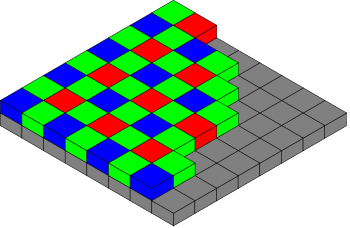
\includegraphics[width=0.35\textwidth]{figures/Bayer_pattern.png}
      \caption{Filtro de Bayer típico de un sensor CMOS-APS. Por cada 4 pixeles 2 son verdes, 1 es rojo y 1 es azul.
        El color verde es utilizado dos veces debido a la sensibilidad al verde del ojo humano.}
      \label{fig:bayer}
    \end{figure}

    \subsection{librería raspiraw}
    Para la adquisicón de datos se utilizó la librería {\it raspiraw}\cite{raspiraw} debido a la rapidez con la que se toman los datos.
    En el apéndice~\ref{sec:ap_alternatives} se muestran otras alternativas que son más lentas para la toma de datos,
    pero que pueden resultar más simples y sencillas de implementar.

    %   Hablar sobre los parámetros que se le pueden variar

    %%%%%%%%%%%%%%%%%%%%%%%%%%%%%%%%%%%%%%%%%%%%%%%%%%%%%%%%%%%%%%%%%%%%%%%%%%%%%
    
    \section{Resultados}
    Para probar el correcto funcionamiento de la librería, se utilizó el poder de procesamiento en dos aplicaciones diferentes.
    Una de ellas consistió en detectar Rayos Cósmicos, y la otra la de observar los picos $K_{\alpha}$ y $K_{\beta}$ de diferentes elementos.
    
    \subsection{Medición de Rayos Cósmicos}

    \subsection{Medición de picos $K_{\alpha}$ y $K_{\beta}$}

    \subsubsection{Cobre}

    \subsubsection{Aluminio}

    \subsubsection{Hierro}

    \subsubsection{Calcio}
    
    %%%%%%%%%%%%%%%%%%%%%%%%%%%%%%%%%%%%%%%%%%%%%%%%%%%%%%%%%%%%%%%%%%%%%%%%%%%%%
    \section{Conclusiones}
    
  

    %%%%%%%%%%%%%%%%%%%%%%%%%%%%%%%%%%%%%%%%%%%%%%%%%%%%%%%%%%%%%%%%%%%%%%%%%%%%%
    \section{Referencias}\label{}
    
    \bibliographystyle{siam}
    \bibliography{bibliography}
    
    %\bibliographystyle{prsty}
    %\begin{thebibliography}{99}
    %\bibitem{lane}Lane, David W., X-ray imaging and spectroscopy using low cost COTS CMOS sensor
    %  - Nuclear Instruments and Methods in Physics Research B - Elsevier[Septiembre 2011]
    %  Physics - 1st Edition, Academic Press,  [1966]
    %\bibitem{melissinos2003}Melissinos, A.C., Napolitano, J.,  Experiments in Modern
    %  Physics - 2nd Edition, Academic Press,  [2003]
    %\bibitem{bevington2003}Bevington and Robinson, Data Reduction and
    %  Error Analysis for the Physical Sciences - 3rd Edition, McGraw-Hill,
    %  [2003]
    %\bibitem{pritchard1990}Professor D. Pritchard, Personal Communication
    %\end{thebibliography}
    
    
    %%%%%%%%%%%%%%%%%%%%%%%%%%%%%%%%%%%%%%%%%%%%%%%%%%%%%%%%%%%%%%%%%%%%%%%%%%%%%
    \begin{acknowledgments}
    Se agradece la colaboración de Xavier Bertou por la experiencia brindada y por
    acompañar el trabajo en forma constante.

    A Miguel Sofo por la disponibilidad y por su flexibilidad a la hora de trabajar

    % A Geraldina Gulop  ¿?
    \end{acknowledgments}
    
    %%%%%%%%%%%%%%%%%%%%%%%%%%%%%%%%%%%%%%%%%%%%%%%%%%%%%%%%%%%%%%%%%%%%%%%%%%%%%
    \clearpage
    \appendix
    
    %%%%%%%%%%%%%%%%%%%%%%%%%%%%%%%%%%%%%%%%%%%%%%%%%%%
    \section{Alternativas a Raspiraw}\label{sec:ap_alternatives}
    
    \section{Documentación de la librería}\label{sec:ap_doc}

    \subsection{rawImages}\label{sec:ap_doc:rawImages}

    \subsection{rawEvent}\label{sec:ap_doc:rawEvent}

    \subsection{rawFilters}\label{sec:ap_doc:rawFilters}


    \end{document}
    